\documentclass{article}

% [jh] hi :)

% if you need to pass options to natbib, use, e.g.:
%     \PassOptionsToPackage{numbers, compress}{natbib}
% before loading neurips_2024


% ready for submission
\usepackage[preprint]{neurips_2024}


% to compile a preprint version, e.g., for submission to arXiv, add add the
% [preprint] option:
%     \usepackage[preprint]{neurips_2024}


% to compile a camera-ready version, add the [final] option, e.g.:
%     \usepackage[final]{neurips_2024}


% to avoid loading the natbib package, add option nonatbib:
%    \usepackage[nonatbib]{neurips_2024}


\usepackage[utf8]{inputenc} % allow utf-8 input
\usepackage[T1]{fontenc}    % use 8-bit T1 fonts
\usepackage{url}            % simple URL typesetting
\usepackage{booktabs}       % professional-quality tables
\usepackage{amsfonts}       % blackboard math symbols
\usepackage{nicefrac}       % compact symbols for 1/2, etc.
\usepackage{microtype}      % microtypography
\usepackage{xcolor}         % colors
\usepackage{lipsum}

\usepackage{amsmath}
\usepackage{amssymb}
\usepackage{mathtools}
\usepackage{enumitem}

\usepackage{amsthm}

\usepackage{multirow}       % multirow

\usepackage{url}
\usepackage[utf8]{inputenc} % allow utf-8 input
\usepackage[T1]{fontenc}    % use 8-bit T1 fonts
\usepackage[breaklinks]{hyperref}      % hyperlinks

\usepackage{booktabs}       % professional-quality tables
\usepackage{amsfonts}       % blackboard math symbols
\usepackage{amsmath}
\usepackage[mathscr]{euscript}
\usepackage{amssymb}
\usepackage{mathtools}
\usepackage{amsthm}
\usepackage{nicefrac}       % compact symbols for 1/2, etc.
\usepackage{microtype}      % microtypography

%\usepackage{wrapfig}
\usepackage{graphicx}
\usepackage{xcolor}      % colors


\usepackage{caption}
\usepackage{multirow,makecell}

\usepackage{xspace}
\usepackage{subcaption}

\usepackage{algorithm}
\usepackage{algorithmic}
\usepackage{wrapfig}



 %\newcommand{\theHalgorithm}{\arabic{algorithm}}

\newcommand{\newstuff}[1]{{\color{blue}#1}}

% if you use cleveref..
\usepackage[capitalize,noabbrev]{cleveref}



%%%%%%%%%%%%%%%%%%%%%%%%%%%%%%%%
% THEOREMS
%%%%%%%%%%%%%%%%%%%%%%%%%%%%%%%%
\theoremstyle{plain}
\newtheorem{theorem}{Theorem}[section]
\newtheorem{proposition}[theorem]{Proposition}
\newtheorem{lemma}[theorem]{Lemma}
\newtheorem{corollary}[theorem]{Corollary}
\theoremstyle{definition}
\newtheorem{definition}[theorem]{Definition}
\newtheorem{assumption}[theorem]{Assumption}
\theoremstyle{remark}
\newtheorem{remark}[theorem]{Remark}


\title{Hogwild! Inference: \\ Parallel LLM Generation via  Concurrent Attention}


% The \author macro works with any number of authors. There are two commands
% used to separate the names and addresses of multiple authors: \And and \AND.
%
% Using \And between authors leaves it to LaTeX to determine where to break the
% lines. Using \AND forces a line break at that point. So, if LaTeX puts 3 of 4
% authors names on the first line, and the last on the second line, try using
% \AND instead of \And before the third author name.


\author{%
  \!\!\!Gleb Rodionov$^{\dagger\,*}$\\
  %$^{Equal contribution} $\,$ 
  %\thanks{Corresponding author: \texttt{rodionovgleb@yandex-team.ru}} \\
  \!\!\!Yandex \\
  \And
  \!\!\!Roman Garipov$^*$ \\
  \!\!\!HSE University, Yandex \\ ITMO University \\
  \And
  \!\!\!Alina Shutova$^*$ \\
  \!\!\!HSE University, Yandex \\
  \And
  \!\!\!George Yakushev$^*$ \!\!\! \\
  \!\!\!HSE University, Yandex\!\!\! \\
  \And
  Vage Egiazarian  \\
  IST Austria \\
  \And
  Anton Sinitsin \\
  Yandex\\
  \And
  Denis Kuznedelev \\
  Yandex \\
  \And
  Dan Alistarh$^\ddagger$\\% \thanks{Senior author}\\
  IST Austria\\
}


\begin{document}



\maketitle


\vspace{-8px}\begin{abstract}
    Large Language Models (LLMs) have demonstrated the ability to tackle increasingly complex tasks through advanced reasoning, long-form content generation, and tool use.
    Solving these tasks often involves long inference-time computations.
    In human problem solving, a common strategy to expedite work is collaboration: by dividing the problem into sub-tasks, exploring different strategies concurrently, etc. Recent research has shown that LLMs can also operate in parallel by implementing explicit cooperation frameworks, such as voting mechanisms or the explicit creation of independent sub-tasks that can be executed in parallel. However, each of these frameworks may not be suitable for all types of tasks, which can hinder their applicability.
    In this work, we propose a different design approach: \textit{we run LLM ``workers'' in parallel , allowing them to synchronize via a concurrently-updated attention cache and prompt these workers to decide how best to collaborate.} Our approach allows the instances to come up with their own collaboration strategy for the problem at hand, all the while ``seeing'' each other's partial progress in the concurrent cache.
    We implement this approach via \textbf{Hogwild! Inference:} a parallel LLM inference engine where multiple instances of the same LLM run in parallel \textbf{with the same attention cache}, with ``instant''  access to each other's generated tokens.\footnote[1]{Our implementation is available at \url{https://github.com/eqimp/hogwild_llm}.} Hogwild! inference takes advantage of Rotary Position Embeddings (RoPE) to avoid recomputation while improving parallel hardware utilization.
    We find that modern reasoning-capable LLMs can perform inference \textit{with shared Key-Value cache} out of the box, without additional fine-tuning.
    
    % We see Hogwild! Inference is only one example in a class of efficient reasoning algorithms based on modern LLMs. Let's see how we can collaborate!
\end{abstract}

\def\thefootnote{$\dagger$}\footnotetext{Corresponding author: \texttt{rodionovgleb@yandex-team.ru}.\quad $^*$ Equal contribution. \quad $\ddagger$ Senior author.} \def\thefootnote{\arabic{footnote}}


\vspace{-5px}\section{Introduction}\label{sect:intro}\vspace{-5px}

\begin{figure}[t]
    \centering
    \vspace{-20px}
    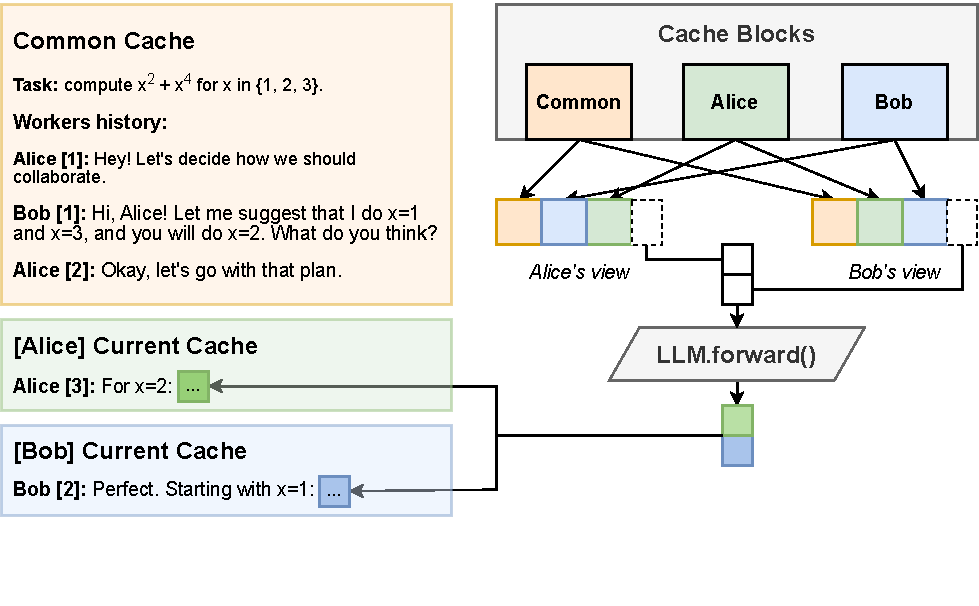
\includegraphics[width=0.9\linewidth, height=215px]{resources/figure1_cropped.pdf}\vspace{-20px}
    \caption{An intuitive explanation of Hogwild!\! Inference, with 2 workers generating in parallel and 3 shared cache blocks. Each color denotes a cache block. \href{https://github.com/eqimp/hogwild_llm/tree/main?tab=readme-ov-file\#demo}{See it in action (example generation)}.}
    \label{fig:teaser}\vspace{-20px}
\end{figure}

A recent trend allowing for further progress in Large Language Models is to leverage their ability to improve performance via additional inference-time computations~\citep{challenging_bigbench_solved_with_cot_Suzgun2022ChallengingBT,scaling_test_time_snell2024scaling,beeching2024scalingtesttimecompute,muennighoff2025s1}. This includes improved reasoning~\citep{cot_wei_2022,zero_shot_cot_Kojima2022LargeLM,auto_cot_Zhang2022AutomaticCO,three_of_thought,verify_step_by_step}, long-form generation~\citep{Bai2024LongWriterU1} and interacting with external tools~\citep{Schick2023ToolformerLM,Qin2023ToolLLMFL,Yao2022ReActSR,Shen2023HuggingGPTSA}. Modern LLM-based services have capabilities for long-form reasoning~\citep{openai_o1,googledeepmind2025gemini25thinking,AnthropicClaude3.7Sonnet}. At the same time, several highly capable reasoning LLMs have recently been released to the public ~\cite{deepseek_r1,qwq32b,qwen2,touvron2023llama,dubey2024llama, muennighoff2025s1,ye2025limoreasoning}.

Using these models to solve complex problems often requires long sequential computations, that is, generating text token-by-token. However, many reasoning problems are not sequential. Leveraging this intuition, several recent works propose parallel inference strategies that allow multiple LLMs to solve a problem faster or more accurately via some form of collaboration~\citep{Wang2022SelfConsistencyIC,ning2024skeletonofthought}.
In the simplest case, multiple LLMs can attempt the problem independently, then vote~\citep{Wang2022SelfConsistencyIC} or cross-reference their results~\citep{du2024improving,wang2024mixture} to improve correctness. A parallel line of work allows the LLM to divide the problem into multiple independent sub-tasks that are then solved in parallel and merged, producing the final solution~\citep{ning2024skeletonofthought, kim2024llm, jin2025learningpromisescalinglanguage}. These parallel inference strategies can improve quality and efficiency, taking advantage of parallelism in modern hardware.

Unfortunately, no single collaboration strategy is universally effective. For instance, solving a problem in independent parallel ``threads'' can be inefficient when one of the threads requires longer generation than the rest, resulting in most of the agents waiting for a straggler and wasting compute~\citep{Wang2022SelfConsistencyIC,wang2024mixture}. In turn, inference with independent sub-tasks only works if the problem can immediately be split into these sub-tasks. Furthermore, if one of the agents discovers that the original plan is flawed, they will be unable to re-plan~\citep{ning2024skeletonofthought,ding2025dynamicparalleltreesearch}, potentially solving sub-tasks that are no longer necessary~\citep{jin2025learningpromisescalinglanguage}.

This runs in contrast to how human reasoners collaborate. Instead of strict adherence to a fixed collaboration strategy, the way human problem solvers may interact is very dynamic, including re-plannning on the fly, abandoning some tasks half-way and switching to a more promising approach, discussing or debating strategy if the initial plan failed. While this type of collaboration is harder to define, it offers greater flexibility and can be more efficient if the participants are cohesive enough~\cite{Hutchins1995, EntinSerfaty1999}.

In this work, we try to apply the same principle to artificial reasoners. Since modern LLMs can already reason and plan~\citep{zhou2024selfdiscover,meta_reasoning_gao2024,wang-etal-2024-meta}, we hypothesize that they can benefit from dynamic interaction between different instances, during which they can develop their own collaboration strategy for the problem at hand.


% Recent works have shown that modern reasoning LLMs are also capable of meta-reasoning --- reasoning how to reason~\citep{zhou2024selfdiscover,meta_reasoning_gao2024,wang-etal-2024-meta}. We hypothesize that they will also be capable at reasoning about how to reason \textit{together}.

To test this hypothesis, we propose Hogwild! Inference --- a parallel LLM inference protocol with no pre-defined framework of collaboration.\footnote[2]{Our approach is loosely inspired by Hogwild! SGD ~\cite{NIPS2011_218a0aef}, an optimizer that runs updates asynchronously and applies each update as soon as it is computed. The exclamation mark is part of the original name~\citep{hogwild_exclamation_mark}.}
Instead of choosing how LLMs should interact ahead of time, we allow them to generate tokens in parallel and ``see'' each other's progress (tokens) \textbf{immediately as they are generated}.
We then prompt the LLM ``workers'' to decide their next course of action by themselves, given the latest actions from others: whether this means solving parallel sub-tasks, cross-verifying each other, discussing strategy, or pivoting to a new plan.

To enable this type of on-the-fly collaboration, Hogwild! Inference runs multiple instances of the same LLM \emph{over the same weights}, but with a \emph{custom Key-Value cache} that shares token representations between workers, allowing concurrent cross-attention. 

Specifically, instead of re-computing Key-Value representations for each worker, we keep track of individual worker KV memories and ``stitch them together'' in a different order for each worker, adjusting for their position embeddings (see Figure \ref{fig:teaser} for an illustration).

We test Hogwild!\! Inference with modern open-source LLMs and find that existing reasoning-capable models, such as QwQ~\citep{qwq32b} and DeepSeek-R1~\citep{deepseek_r1}, can already ``reason about coordinating''. More concretely, we observe that concurrent agents can formulate and follow plans, adapt when the initial plan has failed, point out each other's errors, and use each other's key observations. When prompted to check if they are doing redundant work --- e.g., when one LLM instance is doing a sub-task that is already done by another, or solving a problem that is no longer relevant after a change of plan --- they can often (but not always) detect redundancy and pivot to a different strategy.

In this preliminary study, we build on this observation to test several memory layouts for collaborative inference: i) a naive layout where each instance writes its progress in a contiguous chunk, ii) a chat-like layout, where each instance can write its progress in a private buffer, then periodically commit it to a shared memory for others to see, and iii) a hybrid strategy, where instances use a shared chat-like history \textit{and} can see each other's current message before it is sent. 


We evaluate Hogwild! inference on mathematical problems requiring long-chain reasoning to compare the effectiveness of different memory layouts. Our preliminary experiments show that, across all mentioned cache configurations, parallel instances can consistently maintain their own reasoning paths while dynamically incorporating progress from other instances. Additionally, these instances exhibit signs of emerging collaborative behavior, adapting their interactions based on the given problem.


Our preliminary results suggest that parallel inference with a shared Key-Value cache may offer a promising approach to enable effective collaboration between multiple LLM instances.


% no need to write contributions, but they are:
% - Hogwild! inference framework
% - RoPE stitching - a technique for inference with shared cache
% - evaluating different caching strategies on multiple benchmarks and finding whatever we find there
% - analysis? [not by early arxiv; though, we can show examples]
% - prompts, etc
% - a flexible inference algorithm that is available online


\vspace{-5px}\section{Background}\label{sect:background}\vspace{-5px}

% \subsection{Parallel Inference Strategies}\label{sect:background_parallel_infernece}

Recent works propose a large number of frameworks for parallel reasoning and tool use that vary across several axes: how the parallel instances are organized together, what they exchange, and how often \citep{TTSsurvey}. In this section, we give a brief summary of these methods.

\paragraph{Discussion \& aggregation.} The simplest way to parallelize chain-of-thought reasoning is Self-Consistency~\citep{Wang2022SelfConsistencyIC}, where multiple LLM instances reason independently, then vote on the final solution. This approach was later extended in~\cite{du2024improving}, who replace independent voting with text-based communication rounds. Subsequent works in this field combine multiple LLM types~\citep{wang2024mixture} and scales to more agents~\cite{li2024moreagents}. Another line of work introduces specialized ``roles'' such as the Debugger~\citep{talebirad2023multiagent}, Examiner~\citep{cohen-etal-2023-lm}, Math Teacher~\citep{kong-etal-2024-better}, Judge~\citep{chen-etal-2024-reconcile}, and others, to further augment reasoning.

This type of role-based discussion was shown to greatly improve LLM reasoning factuality for certain tasks~\citep{Wang2022SelfConsistencyIC,du2024improving}, and can even enable multiple weaker LLM agents to collectively outperform state-of-the-art single-agent systems~\citep{wang2024mixture}. However, this improvement is not unique to multiple agents and can be offset with better single-agent prompting~\citep{wang-etal-2024-rethinking-bounds,muennighoff2025s1}. Additionally, these approaches do not necessarily accelerate reasoning,  because at least some of the agents have to solve the entire problem sequentially, and process (re-encode) each other's progress. This creates additional computational overhead, which presents challenges for both runtime and memory efficiency~\cite{wang2024mixture,du2024improving}.

\paragraph{Parallelism for efficiency.} A different line of work leverages multiple LLMs to solve tasks faster in parallel, such as Skeleton-of-Thought (SoT)~\citep{ning2024skeletonofthought}. SoT begins by running a single LLM to outline a plan for solving the problem with independent sub-tasks, then launches parallel LLM instances for each sub-task. Subsequent works propose more complex parallelism strategies such as dynamic parallel tree search~\citep{ding2025dynamicparalleltreesearch} or a single agent spawning asynchronous sub-tasks that are done by background LLM ``threads''~\citep{jin2025learningpromisescalinglanguage}. For problems that involve function calling, these functions can also run in parallel~\citep{kim2024llm,gim2024asynchronousllmfunctioncalling}.

These techniques are known to substantially accelerate inference for problems that fit their type of parallelism. However, we argue that this is also their main limitation: by imposing a specific parallelism strategy, these methods can harm reasoning for problems that do not fit their framework. For instance, when solving a complex reasoning problem, it is often the case that the initial plan turns out to be wrong or incomplete~\citep{muennighoff2025s1,deepseek_r1}, which conflicts with SoT-like methods~\citep{ning2024skeletonofthought,yu2025accelerateparallelizablereasoningparallel} that follow a fixed plan-execute-aggregate schedule. Furthermore, some of the sub-tasks may turn out to be more complicated than originally intended and take up more work, which would cause methods like PASTA~\cite{jin2025learningpromisescalinglanguage} to wait for that single task, whereas a more sophisticated reasoner could adjust the plan to work better in parallel. Note that each individual issue can be amended with a yet another, more complicated parallelism framework, but the sheer number of such cases makes us doubt if this is the right approach. In this work, we propose to allow multiple LLM instances to see each other's progress immediately and interact explicitly or implicitly to devise their own collaboration strategy and adjust it as necessary. We show that, perhaps surprisingly, existing reasoning LLMs already have the ability to leverage this. 


\vspace{-5px}\section{Hogwild! Inference}\label{sect:method}\vspace{-5px}

Our main intuition is that modern LLMs do not need a pre-defined framework for inference-time parallelism: they can organize it by themselves. 
To test this hypothesis, we design a parallel inference protocol where multiple LLM instances can collaborate as flexibly as possible. Instead of assigning each ``worker'' to a specific role or sub-task, we run them in parallel and prompt them to come up with their own means of working together. This approach has two key components: how to run multiple inference threads from the same Key-Value memory, and how to prompt LLM ``workers'' to collaborate over said memory. To that end, we organize this section as follows: we first outline how to perform LLM inference with a shared cache in Section~\ref{sect:method_basic_idea}. Then, in Section~\ref{sect:method_cache_layouts} we describe several possible memory layouts and their implications.
Finally, in Section~\ref{sect:method_prompting}, we describe our strategy for prompting LLMs to collaborate.

\vspace{-5px}\subsection{Concurrent Attention with Shared Key-Value Cache}\label{sect:method_basic_idea}\vspace{-5px}

The core ingredient of Hogwild!\! Inference is a shared Key-Value memory (KV cache) accessible to all workers. The cache consists of several blocks that can be reused between workers, implementing a \textbf{concurrent version of the attention mechanism}~\citep{bahdanau2014neural, vaswani2017attention}. 

Let us first consider the simplest case of Hogwild! Inference with two workers and three cache blocks, as depicted in Figure~\ref{fig:teaser}. The first block contains the prompt, and the other two blocks contain the ``thoughts'' (tokens generated) by workers A and B respectively (denoted Alice and Bob in the Figure).
As workers generate new tokens, they access each other's attention caches as though these were their own previously generated tokens. In Figure~\ref{fig:teaser}, ``Alice'' sees the common prompt, then ``Bob's'' token representations, then her own. In turn, Bob sees the same common prompt, then Alice's token KVs, and his own tokens after that.\footnote[3]{For clarity of exposition, we choose to anthropomorphize the pronouns for these two parallel agents.} 

This creates a discrepancy where the same Key-Value pairs appear on different positions for each worker. Furthermore, the relative distance between the same pair of tokens (e.g., first generated tokens from Alice and Bob, respectively) changes as new tokens are added. While it is possible to re-encode these tokens at their new position, it would cause computation overhead that scales cubically\footnote[4]{If $n$ agents generate one new token each, which is then re-encoded differently for each of these $n$ agents, that each have to attend to $O(n)$ additional tokens, then the total step complexity is $O(n^3)$.}.

Instead of re-encoding the new tokens for other workers, we attempt to reuse existing token representations between workers. However, since these tokens appear at different positions for each worker and step, we need to adjust for their positional embeddings.
Most modern LLMs use Rotary Position Embeddings (RoPE)~\citep{su2021roformer}, where each key and query is rotated to an angle proportional to its absolute position. Prior works have shown that RoPE embeddings can be manipulated through scaling~\citep{rope_scaling} slicing~\citep{streamingllm}, or pruning~\citep{zhang2023h2o}. One very useful property of RoPE embeddings is that they are invariant to parallel shifts in position: if both query and key are rotated by the same angle, the dot product between them will not change. 

In Hogwild!\! Inference, we rely on this property and rotate the entire KV blocks to their position during inference. As shown in Figure~\ref{fig:teaser} (right), the same cache blocks are arranged in different order for each worker, but the relative angle between the tokens within each block stays the same. In other words, the attention score between Alice's last token and her previous tokens does not change from this parallel shift, but she also gains access to Bob's tokens and vice versa.

When generating new tokens in this manner, we perform a forward pass on all workers in parallel, as though they were samples in the same batch.
When processing newly generated tokens, we insert their KV representations at the end of their respective cache blocks, then arrange these cache blocks for each worker. This way, both workers can immediately attend to each other's latest tokens even before they are fully processed by all model layers.
Since re-arranging the cache takes up memory for each worker, we materialize the rearranged Key-Value cache for one attention layer at a time, just-in-time for computation.
% We discuss the technical details further in Appendix~\ref{sect:appendix_implementation}.

\begin{figure}[t]
    \centering
    \vspace{-20px}
    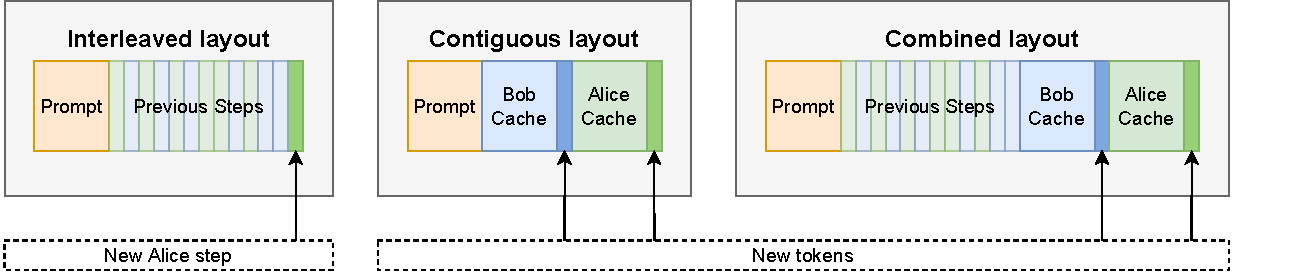
\includegraphics[width=1.045\linewidth,height=82px]{resources/figure2_fixed.pdf}
    \caption{Three cache layouts described in Section~\ref{sect:method_cache_layouts}: interleaved with step-wise synchrony (left), simple contiguous layout (middle) and combined with token-wise synchrony (right). All layouts are made from Alice point of view.}
    \label{fig:layouts}\vspace{-15px}
\end{figure}


\vspace{-5px}\subsection{Cache Layouts}\label{sect:method_cache_layouts}\vspace{-5px}

Now that we established that a cache can be split into blocks and rearranged on the fly, it is reasonable to ask how best to arrange those blocks. In this preliminary study, we consider three such arrangements, shown at Figure \ref{fig:layouts}.

\textbf{Contiguous layout (token-wise)} is the simplest possible layout
where each worker appends to their own sequence blob of tokens and sees other workers' token representations as past keys and values. This layout is inspired by collaborative text editors such as Google Docs or Overleaf.

As described earlier in Section~\ref{sect:method_basic_idea}, each worker arranges the other workers' thoughts in a different order. They see the common prompt cache first, then the caches of all \textit{other} workers (excluding themselves\footnote[5]{When extending this layout to more than 2 workers, each worker sees the key-value memories of everyone except themselves. For instance, given 3 workers A, B, and C, worker B will see a version of the cache that contains the prompt, outputs of workers A and C, and finally, B's own memory. Likewise, A sees B \& C, then A. }), then their own cache as immediate previous tokens. That way, each worker predicts the next token for their own cache.

\textbf{Interleaved layout (step-wise),} which can be seen as analogous to group chat services such as Slack or Discord. In this layout, workers generate tokens \textit{in private} until they finish a reasoning step\footnote[6]{We define a reasoning step as any amount of text that ends with a complete sentence, e.g. a dot or a question mark, and then a double newline (\texttt{"\textbackslash n\textbackslash n"}) in all our experiments, though it may vary by the model.}, then add it to a shared ``history''.
The history contains past reasoning steps of each LLM instance in the order of their completion. Whenever a worker completes a reasoning step, their KV cache entries are moved to the end of the shared history cache block with the proper rotation, then their local cache is reset their local cache for a new step.

In this setup, the workers only see each other's outputs in full steps, not after every token. However, they do not wait for each other to complete their steps. Instead, each worker keeps generating new tokens and occasionally receives additional key-value pairs inserted into its cache.

\textbf{Combined layout (token-wise)} is a mixture of the first two.
The LLM instances 
generate steps that are accumulated in a shared history, as in the interleaved layout. However, they do not generate these steps in private, but can instantly see each other's current progress, as in the contiguous layout.

We can view the first two layouts as ablated versions of this combined one: the contiguous layout lacks the shared history, and the interleaved layout lacks immediate synchronization. We compare these three layouts empirically in Section~\ref{sect:experiments} to better quantify the effect of each design choice.




\vspace{-5px}\subsection{Prompting to Collaborate}\label{sect:method_prompting}\vspace{-5px}

The shared key-value cache inference we described above \textit{allows} modern LLMs to access each other's tokens and reason collaboratively. However, even though modern LLMs can reason about how to collaborate, there is no guarantee it will actually do that without being prompted. As with any desired LLM behavior, it can be achieved in two ways: we can either train a model to generate tokens collaboratively, or prompt it in-context. In this work, we focus on the latter approach to make Hogwild! inference easier to generalize for new models and tasks.

Our current prompting strategy consists of three parts:\begin{enumerate}
    \item \textbf{System prompt:} we describe the ``rules'' of how shared cache layout operates;
    \item \textbf{Partial in-context examples:} we provide excerpts that demonstrate basic cross-instance collaboration --- e.g. when one worker notices that they are working on a task that becomes redundant because of the recent updates from another worker.
    \item \textbf{Inserting s1-like collaboration prompts:} every few steps, we prompt the worker with \textit{``Wait, am I doing redundant work? (yes/no):''} at the beginning  of a new paragraph. This strategy is inspired by \cite{muennighoff2025s1}.
\end{enumerate}

The latter s1-like prompts present a curious case. We often found that, when dealing with LLMs that are pre-trained on reasoning, an agent can  become too ``focused'' on what it is generating currently and fails to notice that another instance has found a mistake or solved their problem earlier. However, then asked directly, they can spot the redundant work and change their approach.

Overall we found that, when prompted this way, LLMs 
often (but not always) detect if what they are doing is redundant, and can reason about what is the best course of action. %We report our current prompts in Appendix~\ref{sect:appendix_prompts} and provide several examples in Appendix~\ref{sect:appendix_examples}. 

Note, however, that these prompts are not a perfect solution to elicit collaborative reasoning, and that we do not claim that they are the optimal way to do so. They are merely one approach that works to a reasonable extent (see Section~\ref{sect:experiments}). An interesting direction for future work is to try and induce collaborative reasoning through different means, such as supervised fine-tuning or reinforcement learning. Once we know that the LLMs \textit{can} reason together, the next milestone is for them to do so consistently.

% This type of inference allows LLMs to re-enact any existing collaboration strategy, such as Skeleton-of-Thought~\cite{ning2024skeletonofthought} or Self-Consistency~\citep{Wang2022SelfConsistencyIC}, but also invent new strategies and alternate between them, e.g. after noticing a mistake or an interesting alternative in another LLM's ``thoughts''.
% We implement this type of concurrent cross-attention with a special type of Key-Value cache that keeps track of each worker's token representations and combines them on the fly for each worker, adjusting their position embeddings.
% To enable this kind of inference, we need to allow multiple LLM agents to attend to each other's tokens concurrently as they are generated. If done naively, it would require either re-encoding those tokens multiple times as they are ``shifted'' to new positions, or pre-allocating a fixed window of positions for each LLM instance, which would result in gaps between them.
% If done naively, it would require each instance to copy and re-encode tokens from other instances as new ones are added and shift in position, slowing down computation. To address this problem, we propose an alternative strategy where each instance's memory is instantly available to others.
% to study this test case, we propose Hogwild!\! Inference - a novel inference framework where multiple instances of the same LLM run concurrently, with instructions to invent their own strategy for collaborating, and synchronizing via a shared attention cache.
% Specifically, in Hogwild!\!inference, all LLM instances share the same Key-Value memory. Thus, at a given point in time, an LLM ``worker'' can see the others' progress in terms of items that populate the cache. To ensure efficiency, the cache is ``stitched together'' in different ways for each LLM instance using a procedure we call RoPE stitching. This allows Hogwild! Inference to be integrated easily into modern LLM inference libraries, where it can be implemente as batched inference with a custom Key-Value Cache. We release our reference implementation online\footnote{TODO}.




% HERE BE DRAGONS


% In order to allow for a flexible collaborative inference framework, we need a way to allow agents to see each other's workings, so they may exchange intermediate results, see each other's progress and pivot their actions as necessary. To reduce the communication delays, Hogwild! inference needs LLMs to immediately see each other's tokens as they are generated. However, when done naively, this would require a lot of recomputation: every time one LLM instance generates a token, we need to copy it to others' attention memory, which would in turn cause their own tokens to shift by one position. While it is possible to simply re-encode these tokens at their new position, doing so would cause computation overhead that scales cubically\footnote{$n$ agents generate one new token each, which is then re-encoded differently for each of these $n$ agents, that each have to attend to $O(n)$ additional tokens, which means that the total step complexity is $O(n^3)$.} with the number of agents and needs additional VRAM.
% To model these dependencies directly, we would need to re-encode tokens from other instances as they shift in position and new ones are added. However, that would
% as new ones are added and shift in position, slowing down computation. To address this problem, we propose an alternative strategy where each instance's memory is instantly available to others.

% TODO\begin{enumerate}
%     \item general idea, cache is divided into blocks, some blocks are reused between workers. Each worker appends to the last cache in their structure. Mention that due to RoPE and different positions, cache stitching needs special treatment that is discussed in Section~\ref{sect:method_implementation}.
%     \item cache layout 1 - contiguous. Inspired by concurrent work on collaborative document editor (e.g. Google Docs, Overleaf, etc)
%     \item cache layout 2 - interleaved. similar to concurrent work on a chat room (e.g. Discord, Slack, etc)
%     \item combined cache layout - interleaved history, but workers can see current step like in google docs. Not sure if useful to humans, but LLMs are not us.
%     \item discuss synchronization - by token, by step, every k steps, can be important in distributed setup - MOVE TO DISCUSSION
%     \item Schemes for at least one , but better - both inference layouts, link to video in caption
% \end{enumerate} 



\section{Initial Experiments}\label{sect:experiments}



In this section, we conduct an initial evaluation of Hogwild! Inference under different conditions. We run our main evaluations with the \textbf{QwQ-32B} model\footnote[7]{\url{https://huggingface.co/Qwen/QwQ-32B}} and consider two evaluation setups: simple synthetic tasks that require minimal communication and a more challenging set of reasoning problems that require more complex collaboration patterns.

\paragraph{Sanity checks with synthetic tasks:} 
Before we try our approach on more challenging tasks, we test if Hogwild!\! Inference is capable of basic collaboration.
For this purpose, we construct a toy problem set where each sample contains 5 questions from the GSM8k test set~\cite{cobbe2021gsm8k}. To decouple the effects of parallelism, we filter the questions that the model could solve within 256 generated tokens. We evaluate on 100 sets with 3 non-intersecting problems each. The LLM is prompted to solve each problem and return comma-separated values\footnote[8]{\texttt{"Solve these problems and return comma-separated answers \textbackslash boxed\{answer1,..., answer5\} :\textbackslash n 1. \{task1\}\textbackslash n 2. \{task2\}\textbackslash n 3. \{task3\}\textbackslash n 4. \{task4\}\textbackslash n 5. \{task5\}"}}. We report the average fraction of problems solved, e.g. if the LLM solved 4 out of 5 tasks in a given set, it will get a score of 0.8 for that sample.

For this simple sanity check, we compare two settings: sequential generation and Hogwild! Inference with the \textit{combined cache layout} for 2 and 4 workers. In each case, we control for the total number of forward passes the LLM is allowed to perform. If the LLM returns the full comma-separated answer within the budget, we count the accuracy based on each individual answer.



Note, however, that the LLM does not always produce the answer in time, especially with a tight budget. To extract the answers from partial reasoning, we take all outputs produced by the method and insert a special prompt\footnote[9]{\texttt{"\textbackslash n\textbackslash nWait, given the limited time, I have to give an answer right now. Conside- ring all my previous attempts, I have to conclude that the 5 answers are \textbackslash boxed\{"}} that forces the model to return the answer early. With QwQ-32B, we observe that the model almost always returns answers correctly if they are present, and if not, it guesses or refuses to answer (\texttt{unknown}, \texttt{n/a} or similar). We let the model compile the answer with greedy decoding for at most 32 tokens without parallelism. When extracting answers from Hogwild! Inference, we let the final model view all generated tokens from each worker\footnote[10]{This is equivalent to viewing the problem from the perspective of the last worker, e.g. Bob if there are two.}.

\begin{wrapfigure}{r}{0.4\textwidth}
  \vspace{-20px}
  \begin{center}
    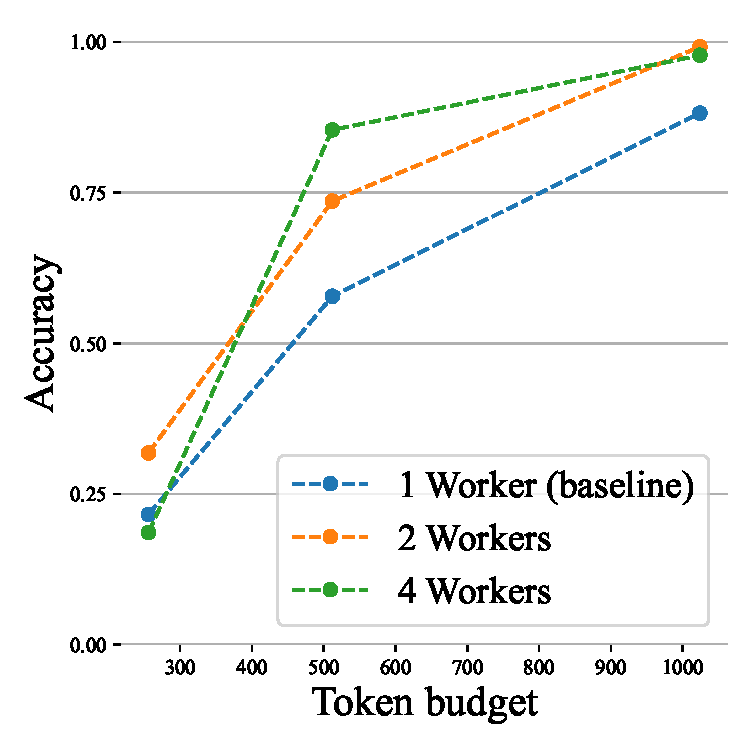
\includegraphics[width=0.4\textwidth]{resources/method_comparison_gsm8k.pdf}
  \end{center}
  \vspace{-10px}
  \caption{Evaluation results for synthetic problems with 5 GSM8k questions each.}\vspace{-10px}
  \label{fig:results_gsm8k}

\end{wrapfigure}


The results in Figure~\ref{fig:results_gsm8k} demonstrate that the parallel workers under Hogwild! Inference can indeed collaborate. When inspecting the generated traces, we found that the workers almost always spend the first few steps ``discussing'' how to split the work, then execute the assigned tasks. If one of the workers finishes their task early and there are no other tasks left, they typically either stall or double-check other workers' tasks. Note also that the accuracy with 4 workers is slightly higher than what can be extrapolated from 256 tokens per task. Upon closer examination, we found that many of the tasks require much fewer than 256 tokens, and when 4 workers attempt their tasks, the worker that finishes first often (but not always) takes up the remaining task. One anomalous result is when 4 workers have the budget of 256 tokens, where they underperform even the single worker baseline. This is because most of the budget is spent on coordination.

\textbf{LIMO tasks.} Next, we evaluate Hogwild! Inference on a more challenging problem set where there is no clear pattern of collaboration. We adopt the dataset from~\cite{ye2025limoreasoning} that contains mathematical problems that require thousands of tokens to solve reliably. Unlike our synthetic tasks, the problems in that dataset often do not have an obvious collaboration strategy ahead of time. However, as the LLM starts its reasoning chain, it often discovers situations where there are multiple cases or equations to solve in parallel, or alternatively, multiple possible strategies to solve a single problem. To evaluate on this dataset, we take 512 samples from the original dataset\footnote[11]{We used \url{https://huggingface.co/datasets/GAIR/LIMO}} (slightly over a half of the full dataset) and use the remaining samples for development.

Here, we compare the three Hogwild! cache layouts described in Section~\ref{sect:method_cache_layouts}. We also evaluate three baselines: i) a simple baseline that performs reasoning up to a given budget and is expected to provide the answer in \texttt{\textbackslash boxed\{ \}}. ii) an improved baseline where we prompt the LLM to produce the final answer if it did not generate one yet (same as above, \texttt{"Wait, given limited time ..."}, except \texttt{"5 answers"} $\longrightarrow$ \texttt{"the answer"}, generate at most 8 tokens) and iii) a naive parallel strategy inspired by~\cite{Wang2022SelfConsistencyIC}, where 2 workers both attempt to solve the task without communication, then we extract the answer with the same prompt as above.


We summarize our results in Figure~\ref{fig:results}: even in this more challenging task, Hogwild\! Inference with multiple workers can solve the problems faster than a single thread. Both interleaved cache and token-wise synchrony seem to contribute to the quality. Without interleaved cache (i.e. Contiguous layout), the workers seem to work well for smaller budgets, but their efficiency drops as they generate more tokens. We hypothesize that, when each worker generated many thousands of tokens, it becomes harder to notice and react to what the other assistant is doing. Conversely, interleaved layout without immediate synchronization performs poorly at small budgets, but then catches up as the workers are allowed to generate more tokens. We attribute this to the fact that, without step-wise synchrony, workers need more ``time'' to converge to a collaboration strategy. We present an illustrative example of the generation process for Hogwild! inference in Appendix~\ref{sect:appendix_examples}. We also report a more detailed accuracy breakdown for different budgets in Appendix~\ref{sect:appendix_extra_plots}.

Note, however, that these are only preliminary experiments that leave out many important questions: what is the impact of the prompting strategy? Does Hogwild!\! Inference work for other problem types (programming, function calling, etc)? Does the model's ability to reason on the problem correlate with how well it collaborates? Additionally, it is curious if we can \textit{train} the model to collaborate better through means such as supervised fine-tuning or reinforcement learning.

\begin{figure}[t]
    \centering
    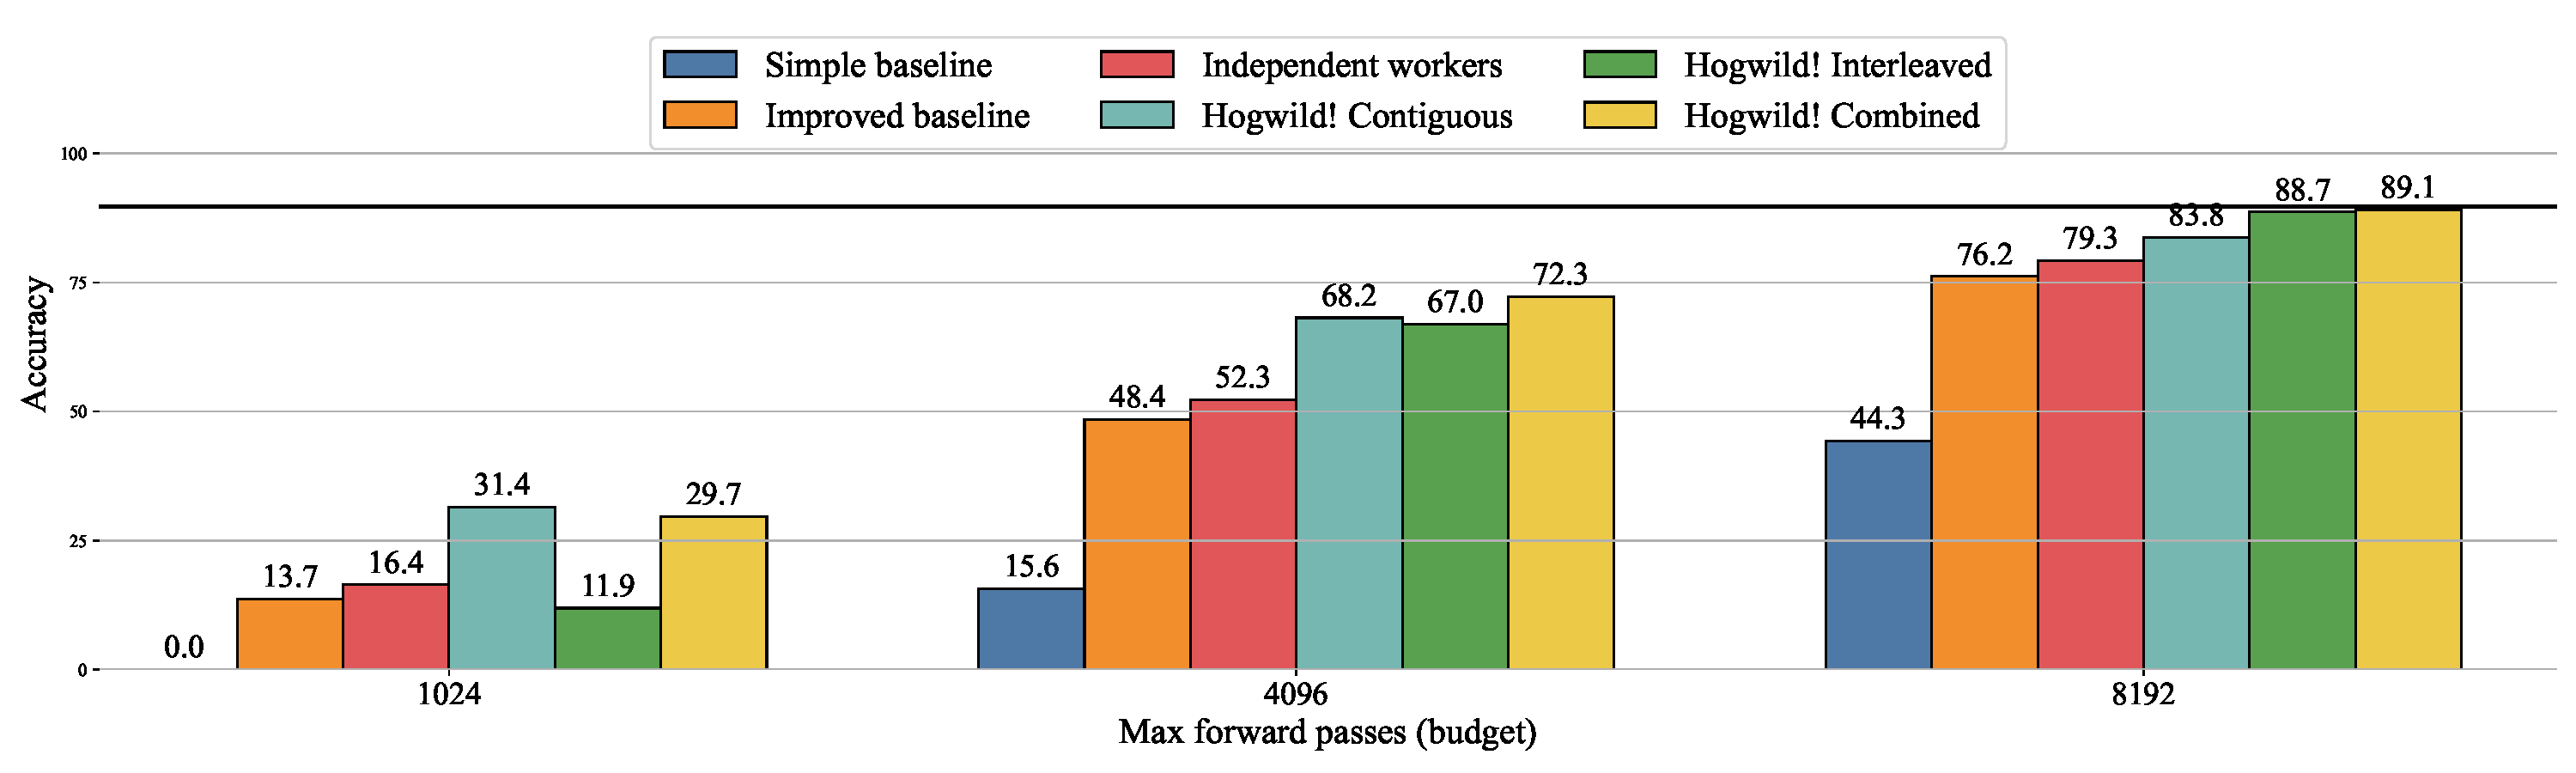
\includegraphics[width=1\linewidth]{resources/graphics.pdf}
    \caption{Evaluation on 512 LIMO tasks. The horizontal black line corresponds to running single-threaded reasoning for 16384 tokens (Accuracy 89.65\%). More budgets in Appendix~\ref{sect:appendix_extra_plots} (Figure~\ref{fig:limo_detailed_plot}).}
    \label{fig:results}
\end{figure}



\section{Discussion}\label{sect:discussion}

In this working paper, we have investigated the ability of reasoning LLMs to implement parallelism in their task solutions when prompted to do so. 
Perhaps surprisingly, our results suggest that LLMs are able to implement such parallelism based on few-shot examples, without specialized fine-tuning: individual ``parallel'' LLM threads can coordinate explicitly, and leverage each other's partial progress in their solutions. 
Beyond demonstrating high-level feasibility, our implementation prototype, called Hogwild! Inference, enables multiple inference threads to concurrently access and update a shared attention cache. Exploiting Rotary Position Embeddings (RoPE), this design has minimal overhead, while improving hardware utilization. 

In future work, we plan to perform a thorough investigation of attention concurrency mechanisms in terms of trading off accuracy vs. parallelism, as well as the impact of supervised fine-tuning for better enabling task parallelism. 
Another consideration is that the effectiveness of Hogwild! Inference may vary  across tasks, requiring a detailed analysis of task-dependent performance. For instance, while reasoning problems that naturally decompose into independent or semi-independent subtasks might readily benefit from Hogwild! inference, tasks requiring strict sequential logic have low potential for parallel gains.
At the same time, parallel inference introduces non-determinism, as the final output could depend on subtle timing interactions between parallel threads. 
We also plan to investigate connections to alternative schemes which enable parallel inference such as speculative decoding~\citep{leviathan2023fast}, or parallel token generation via methods like Medusa~\citep{cai2024medusa} or EAGLE~\citep{li2024eagle}. 


\paragraph{Acknowledgements:} we would like to acknowledge Vladimir Malinovskii for his help with the initial brainstorming, helpful suggestions and suggesting future work directions. We also thank Philip Zmushko for proofreading.

% This observation poses several interesting questions for future research. Now that we know that LLMs are capable of this one-memory-multiple-workers type of inference, what is the best way to arrange their shared memory? Now that we know that reasoning LLMs can cooperate, how can we teach them to collaborate more effectively?


% Passing mention: we are somewhat related to speculative decoding since we both exploit the same inefficiency of inference-time. We can also be combined, e.g. see Medusa, Eagle can do batched SD faster

\bibliography{main}
\bibliographystyle{plainnat}

\newpage
\appendix
% \section{Implementation Matters}\label{sect:appendix_implementation}


% To circumvent this complexity, TODOName avoids re-encoding those tokens. Instead, we manipulate existing token representations to make them reusable between LLM instances. Our approach is inspired by TODO RoPE scaling, H2O, Streaming LLM.



% TODO\begin{enumerate}
%     \item main setup: single GPU, single LLM, this has advantages
%     \item we store cache 'blocks' and stitch them together just in time, one layer at a time
%     \item block position and context can change over time. Normally, it would require re-encoding
%     \item instead, we simply rotate blocks to a new offset just-in-time - which can be done by multiplying them by a pre-determined cos/sin pair - and then concatenate them together - we call that RoPE stitching
%     \item RoPE stitching can potentially be fused into attention computation, but this is future work
%     \item also consider distributed setup, where sync frequency can be important
% \end{enumerate}

% % \begin{figure}[t]
% %     \centering
% %     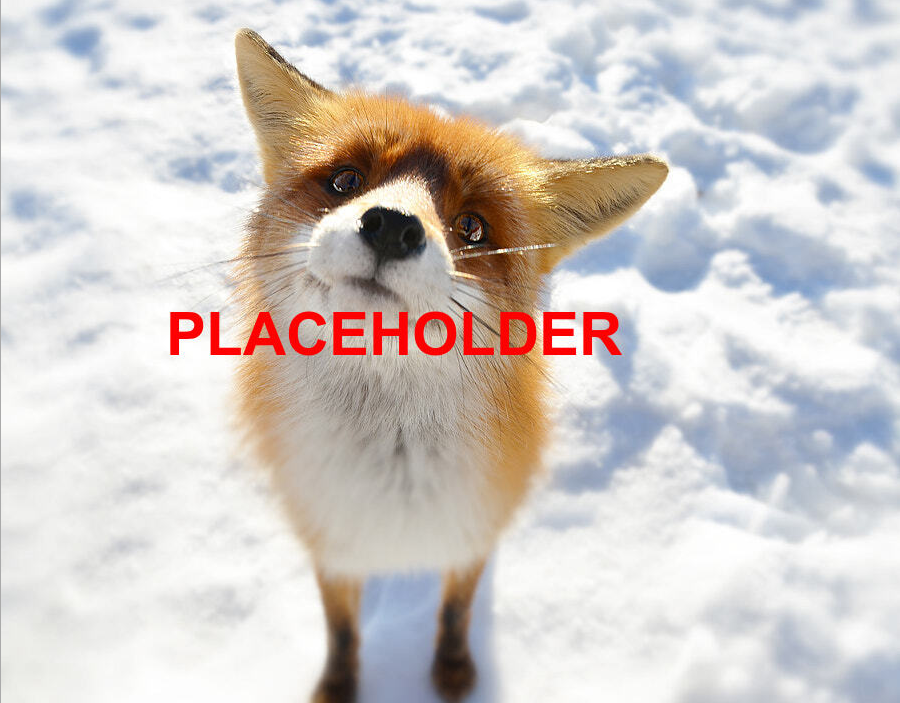
\includegraphics[width=\linewidth, height=150px]{resources/placeholder.png}
% %     \caption{(left) shared cache definition framework used in our reference implementation[TODOclickable] (right) compiling this cache for batched inference with RoPE stitching.}
% %     \label{fig:cache_manager_and_rope_stitching}
% % \end{figure}


% \section{Prompting Details}\label{sect:appendix_prompts}

% TODO HERE BE DRAGONS

% \section{Few-shot examples}\label{sect:appendix_examples}

% TODO HERE BE DRAGONS

\section{Examples}\label{sect:appendix_examples}

In this section, we present a reasoning chain, generated by Hogwild!\! Inference with an interleaved cache layout and token-wise synchronization.
We denote our intervention in model generation in \textit{italics} and highlight worker interactions with \textbf{bold} to enhance readability.
\subsection{Example from LIMO math dataset}\label{sect:appendix_example_1}
\textit{Problem:} For $t = 1, 2, 3, 4$ , define $S_t = \sum_{i = 1}^{350}a_i^t$ , where $a_i \in \{1,2,3,4\}$ . If $S_1 = 513$ and $S_4 = 4745$ , find the minimum possible value for $S_2$

\textit{> Bob [1]: Hi, I'm Bob.} Let me suggest that we first model this as an optimization problem with constraints. We have variables representing the number of each $a_i$ equal to $1,2,3,4$. Let me denote the counts as $n_1,n_2,n_3,n_4$ where $n_1 + n_2 +n_3 +n_4 =350$. Then $S_1=1 n_1 +2n_2 +3n_3 +4n_4 =513$. $S_4=1^4n_1 +2^4n_2 +3^4n_3 +4^4n_4 = n_1 +16n_2 +81n_3 +256n_4=4745$. We need to minimize $S_2= n_1 +4n_2 +9n_3 +16n_4$. So with variables $n_1,n_2,n_3,n_4$ non-negative integers. Since there are three equations and four variables, we can express variables in terms of some parameters and find the minimum $S_2$.

\textit{> Alice [1]: Hi, I'm Alice. Here's how we should do this:} Since we need to minimize $S_2$ given $S_1=513$ and $S_4=4745$, with each $a_i$ being $1,2,3,4$. Let me think of variables $n_1,n_2,n_3,n_4$ as the counts of each number. So $n_1 +n_2 +n_3 +n_4=350$. The first moment $S_1 =n_1 +2n_2 +3n_3 +4n_4=513$. The fourth moment $S_4 =n_1 +16n_2 +81n_3 +256n_4=4745$. We need to minimize $S_2 =n_1 +4n_2 +9n_3 +16n_4$. Let me write down the equations:

Equation 1: $n_1 +n_2 +n_3 +n_4=350$,

Equation 2: $n_1 +2n_2 +3n_3 +4n_4=513$,

Equation 4: $n_1 +16n_2 +81n_3 +256n_4=4745$.

% \textit{> Alice [2]:}  Equation 4: $n_1 +16n_2 +81n_3 +256n_4=4745$.

\textit{> Bob [2]:} \textit{Sanity check: am I doing redundant work? (y/n):} Let me see. \textbf{Alice is setting up the variables and equations. I can proceed to express variables in terms of others. Let me try to subtract equation 1 from equation 2} to get $(n_2 +2n_3 +3n_4)=513-350=163$. So Equation 2 - Equation 1 gives: $(n_2 +2n_3 +3n_4)=163$. Let me call this Equation A.

\textit{> Alice [3]:}  \textbf{Let me also subtract equation 1 from equation 4}: Equation 4 - Equation 1 gives $15n_2 +80n_3 +255n_4 =4745-350=4395$. Simplify this equation by dividing by $5$: $3n_2 +16n_3 +51n_4=879$. Let me call this Equation B.

\textit{...<Bob tried one approach and it did not gave results>...}
% \textit{> Bob [3]:} 1$5n_2 +80n_3 +255n_4 =4395$. Hmm, perhaps we can simplify further. Let me divide by common factors. $15n_2 +80n_3 +255n_4 =4395$. Let me see: $15$ is a common factor for first and third terms: $15(n_2 + 17n_4) +80n_3 =4395$. Hmm, not sure yet. Alternatively, maybe find another relation.

\textit{> Bob [4]:}  Let me note that Equation A: $n_2 =163 -2n_3 -3n_4$. Substitute this into Equation B: 
\textit{...<Bob did math simultaneously with Alice starting from Equation B to derive Equation C>...}
% $3\cdot (163 -2n_3 -3n_4) +16n_3 +51n_4 =879$. Let me compute this:

% $$3\cdot 163 = 489,$$
% $$3\cdot (-2n_3) = -6n_3,$$
% $$3\cdot (-3n_4) =-9n_4,$$
% Thus, equation becomes:

% $489 -6n_3 -9n_4 +16n_3 +51n_4 =879 \to 489 +10n_3 +42n_4 =879 \to 10n_3 +42n_4 = 390 $ divide by $2$ 
$5n_3 +21n_4=195$. \textbf{Same as Alice's Equation C}.

\textit{> Alice [4]:} \textit{Sanity check: am I doing redundant work? (y/n):} Let me see. \textbf{Bob is working on equation B. Let me see if we can express variables in terms of others.} Let me let variables be $n_1,n_2,n_3,n_4$. From Equation A: $n_2 +2n_3 +3n_4 =163$. \textit{...<Alice did math simultaneously with Bob starting from Equation A to derive Equation C>...}
% Let me solve for $n_2$: $n_2 =163 -2n_3 -3n_4$. Substitute this into Equation B: $3\cdot (163 -2n_3 -3n_4) +16n_3 +51n_4 =879$. Let me compute that: $489 -6n_3 -9n_4 +16n_3 +51n_4 =879 \to (489) + (10n_3 +42n_4)=879$. So 1$0n_3 +42n_4 = 879-489=390$.
Simplify this equation by dividing by common factors. Let me see $10$ and $42$ have GCD $2$: divide both sides by $2$: $5n_3 +21n_4=195$. Let me call this Equation C: $5n_3 +21n_4=195$.

\textit{> Bob [5]:} \textit{Sanity check: am I doing redundant work? (y/n):} Yes, \textbf{Alice is already working on equation C. Let me see what else I can do.} 
\textit{...<Bob tried different thing and it did not gave results>...}

% Let me try to express $n_3$ in terms of $n_4$ from equation C: $5n_3 =195 -21n_4 \implies  n_3=(195-21n_4)/5= 39 - (21/5)n_4$. Hmm, so $21n_4$ must be congruent to $195 \mod5$. Since $195 \mod5=0$, so $21n_4$ must be divisible by $5$. Since $21 \mod5=1$, so $n_4 \mod5$ must be $0$. So $n_4$ must be multiple of $5$. Let me let $n_4=5k$, where $k$ is integer $\geq0$. Then $n_3=39 -21\cdot (5k)/5=39-21k$. Wait, wait: $n_4=5k$. So substituting back:

% $$n_3= (195 -21\cdot (5k))/5 = (195 -105k)/5 = 39 -21k.$$

\textit{> Alice [5]:}  Equation C: $5n_3 +21n_4=195$. Let me see possible integer solutions. Let me write this as $5n_3 =195 -21n_4 \implies  n_3 = (195-21n_4)/5$. For $n_3$ to be integer, $195 -21n_4$ must be divisible by $5$. Let me compute $21n_4 \mod5. 21 \mod5=1$, so $21n_4 \mod5 =n_4 \mod5$. Thus, $195 \mod5=0$, so $195 -21n_4 =0 \mod5 \implies  -21n_4 =0 \mod5 \implies  -n_4 =0 \mod5 \implies  n_4 =0 \mod5$. \textbf{Therefore, $n_4$ must be a multiple of $5$.} Let me let $n_4=5k$, where $k$ is a non-negative integer. Then $n_3=(195 -21\cdot (5k))/5 = (195 -105k)/5 =39 -21k$. Since $n_3$ must be non-negative, $39-21k \geq0 \implies  21k \leq39 \implies  k \leq39/21 \approx 1.857$. So $k$ can be $0,1$. Because $k$ must be integer. \textit{...<Alice double checked herself>...}
% Wait, $39/21=1.857$ so $k$ can be $0$ or $1$. Wait, $21\cdot 1=21$, so $39-21=18$, which is positive. If $k=2$, then $39-42=-3 <0$. So $k$ can only be $0$ or $1$. Hmm, so possible $n_4$ is $0$ or $5$. Let me check:

If $k=0$: $n_4=0$, then $n_3=39-0=39$.

\textit{> Bob [6]:} \textit{Sanity check: am I doing redundant work? (y/n):} \textbf{Alice is working on expressing $n_3$ and $n_4$. Let me see if I can find other relations.} \textit{...<Bob tried to find similar equations with no result>...}
% Let me also note that $n_1 =350 -n_2 -n_3 -n_4$ from Equation 1. Since $n_2=163-2n_3-3n_4$ (from Equation A), substituting into $n_1$ gives: $n_1=350 - (163-2n_3-3n_4) -n_3 -n_4 =350-163 +2n_3 +3n_4 -n_3 -n_4=187 +n_3 +2n_4. So n_1=187 +n_3 +2n_4$. So all variables expressed in terms of $n_3$ and $n_4$. Since we have $n_4=5k$, and $n_3=39-21k$. Let me substitute into $n_1$:

% $$n_1=187 + (39-21k) +2\cdot (5k)=187+39-21k+10k=226 -11k.$$


\textit{> Bob [8]:} \textit{Sanity check: am I doing redundant work? (y/n):} \textbf{Alice is handling case1. Let me handle case2 when $k=1$.}

\textit{> Alice [6]:} \textit{Sanity check: am I doing redundant work? (y/n):} Let me proceed. So $n_4$ can be $0$ or $5$. Let me check both possibilities:

Case1: $k=0 \implies n_4=0, n_3=39$. 
\textit{...<Alice did math cheking case1 where $k=0$>...}
% Then $n_2=163-2\cdot 39 -3\cdot 0=163-78=85$. Then $n_1=187 +39 +0=226$. Let me check total variables: $226+85+39+0=350$ <correct>. Check $S_1$: $226\cdot 1 +85\cdot 2 +39\cdot 3 +0\cdot 4=226+170+117+0=513$ <correct>. Check $S_4$:$226 +16\cdot 85 +81\cdot 39 +256\cdot 0=226+1360+3159+0=4745$ <correct>.
So this case is valid.

% \textit{> Alice [7]:}  Wait, let's compute $S_2$ for each case. 

\textit{> Alice [8]:}  For Case1 ($k=0$):
$$S_2 = n_1 +4n_2 +9n_3 +16n_4 =226 +4\cdot 85 +9\cdot 39 +0 =226 +340 +351= 226+340=566;$$
$$ 566+351=917.$$

\textit{> Bob [9]:}  Let me check for $k=1$. \textit{...<Bob did math cheking case2 where $k=1$>...}
% So $n_4=5$, $n_3=39-21\cdot 1=18$. Then $n_2=163 -2\cdot 18 -3\cdot 5=163-36-15=112$. Then $n_1=187 +18 +2\cdot 5=187+18+10=215$. Check total:$215+112+18+5=350$ <correct>. $S_1$:$215 +224 +54 +20=513$ <correct>. $S_4$:$215 +16\cdot 112 +81\cdot 18 +256\cdot 5=215+1792+1458+1280=215+1792=2007; 2007+1458=3465; 3465+1280=4745$ <correct>. So case2 is valid. Now compute $S_2$ for case2: $S_2=215 +4\cdot 112 +9\cdot 18 +16\cdot 5$. $4\cdot 112=448$, $9\cdot 18=162$, $16\cdot 5=80$. Total:$215+448=663$; $663+162=825$; $825+80=905$.
So between the two cases, the minimum $S_2$ is $905$. 

\textit{> Alice [9]:} \textit{Sanity check: am I doing redundant work? (y/n):} \textbf{Bob is checking $k=1$.} Let me compute $S_2$ for both cases. 

\textit{...<Alice validated their approach>...}

\textit{> Bob [10]:} <Bob validated their approach> \textbf{earlier we deduced} $n_4$ must be multiple of $5$ because $n_4 =0 \mod5$. Because $21n_4 =n_4 \mod5$ must be $0$. So yes, only multiples of $5$. Thus only $k=0$ and1. So $905$ is the minimal. 

\textit{> Alice [11]:}  So the minimal $S_2$ is $905$. \textit{...<Alice once again checking answer>...}

\textit{...<Alice and Bob validated their solution checking corner cases>...}

\textit{> Alice [17]:} \textit{Sanity check: am I doing redundant work? (y/n):} Let me confirm with the earlier computations. For $k=1$, $S_2=905$, which matches. So yes. Thus the minimal is $905$. But the problem states that $a_i$ are in $\{1,2,3,4\}$, so the counts must be non-negative integers, which they are in both cases. So the minimal $S_2$ is $905$. Therefore, the answer is \boxed{905}.


\section{Additional LIMO evaluations}\label{sect:appendix_extra_plots}

Here, we report a more detailed breakdown of our evaluation on LIMO tasks from Section~\ref{sect:experiments}. Namely, we consider include additional budgets and arrange our results on a common plot.

\begin{figure}[h]
    \centering
    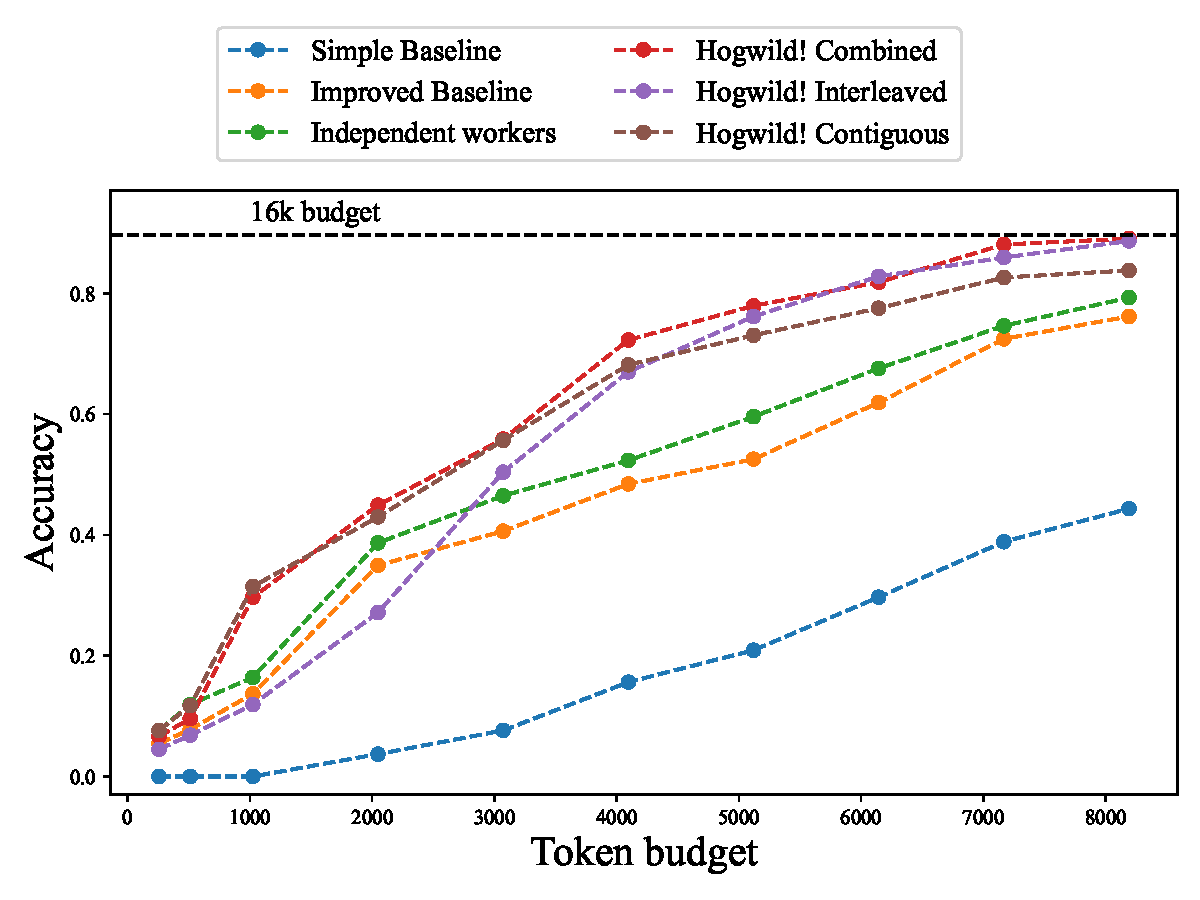
\includegraphics[width=\linewidth]{resources/method_comparison_limo.pdf}
    \caption{Detailed comparison of various parallel inference setups and baselines on LIMO task set, in the same setup as in Section~\ref{sect:experiments}.}
    \label{fig:limo_detailed_plot}
\end{figure}

\end{document}